
\documentclass{beamer}
\usecolortheme{dove}
\setbeamertemplate{navigation symbols}{}
\usepackage{amsmath,amssymb,amsfonts,amsthm, multicol, subfigure, color}
\usepackage{bm}
\usepackage{graphicx}
\usepackage{tabularx}
\usepackage{booktabs}
\usepackage{hyperref}
\usepackage{pdfpages}
\usepackage{xcolor}
\definecolor{seagreen}{RGB}{46, 139, 87}
\definecolor{mustard}{RGB}{234, 170, 0}
\def\independenT#1#2{\mathrel{\rlap{$#1#2$}\mkern2mu{#1#2}}}
\newcommand\indep{\protect\mathpalette{\protect\independenT}{\perp}}
\def\log{\text{log}}
\newcommand\logit{\text{logit}}
\newcommand\iid{\stackrel{\text{iid}}{\sim}}
\newcommand\E{\text{E}}
\newcommand\V{\text{V}}
\renewcommand\P{\text{P}}
\newcommand{\Cov}{\text{Cov}}
\newcommand{\Cor}{\text{Cor}}
\newcommand\doop{\texttt{do}}
\usepackage{stackrel}
\usepackage{tikz}
\usetikzlibrary{arrows,shapes.arrows,positioning,shapes,patterns,calc}
\newcommand\slideref[1]{\vskip .1cm \tiny \textcolor{gray}{{#1}}}
\newcommand\red[1]{\color{red}#1}
\newcommand\blue[1]{\color{blue}#1}
\newcommand\gray[1]{\color{gray}#1}
\newcommand\seagreen[1]{\color{seagreen}#1}
\newcommand\purple[1]{\color{purple}#1}
\newcommand\orange[1]{\color{orange}#1}
\newcommand\black[1]{\color{black}#1}
\newcommand\white[1]{\color{white}#1}
\newcommand\teal[1]{\color{teal}#1}
\newcommand\magenta[1]{\color{magenta}#1}
\newcommand\Fuchsia[1]{\color{Fuchsia}#1}
\newcommand\BlueGreen[1]{\color{BlueGreen}#1}
\newcommand\bblue[1]{\textcolor{blue}{\textbf{#1}}}
\newcommand\bred[1]{\textcolor{red}{\textbf{#1}}}
\newcommand\bgray[1]{\textcolor{gray}{\textbf{#1}}}
\newcommand\bgreen[1]{\textcolor{seagreen}{\textbf{#1}}}
\newcommand\bref[2]{\href{#1}{\color{blue}{#2}}}
\colorlet{lightgray}{gray!40}
\pgfdeclarelayer{bg}    % declare background layer for tikz
\pgfsetlayers{bg,main} % order layers for tikz
\newcommand\mycite[1]{\begin{scriptsize}\textcolor{darkgray}{(#1)}\end{scriptsize}}
\newcommand{\tcframe}{\frame{
%\small{
\only<1|handout:0>{\tableofcontents}
\only<2|handout:1>{\tableofcontents[currentsubsection]}}
%}
}

\newcommand{\goalsframe}{\begin{frame}{Goals of the course}

\begin{itemize}
\item visualize economic inequality with graphs\\that summarize survey data
\item connect theories about inequality to\\quantitative empirical evidence
\item evaluate interventions to reduce inequality
\item conduct data analysis using\\the R programming language
\end{itemize}
\end{frame}}

\usepackage[round]{natbib}
\bibliographystyle{humannat-mod}
\setbeamertemplate{enumerate items}[default]
\usepackage{mathtools}

\title{Studying Social Inequality with Data Science}
\author{Ian Lundberg}
\date{\today}

\begin{document}

\begin{frame}
\begin{tikzpicture}[x = \textwidth, y = \textheight]
\node at (0,0) {};
\node at (1,1) {};
\node[anchor = north west, align = left, font = \huge] at (0,.9) {Studying\\Social Inequality\\with Data Science};
\node[anchor = north east, align = right] (number) at (1,.9) {INFO 3370 / 5371\\Spring 2024};
\node[anchor = north, font = \Large, align = left] at (.5,.5) {\bblue{Course Summary}};
\end{tikzpicture}
\end{frame}

\goalsframe

\begin{frame}{What we did in this course}
\begin{enumerate}
\item Population Sampling
\item Working with Data
\item Describing Inequality
\item Reducing Inequality
\end{enumerate}
leading to your own final projects
\end{frame}

\begin{frame}
\begin{tikzpicture}[x = \textwidth, y = \textheight]
\node at (0,0) {};
\node at (1,1) {};
\node[anchor = west] at (0,.5) {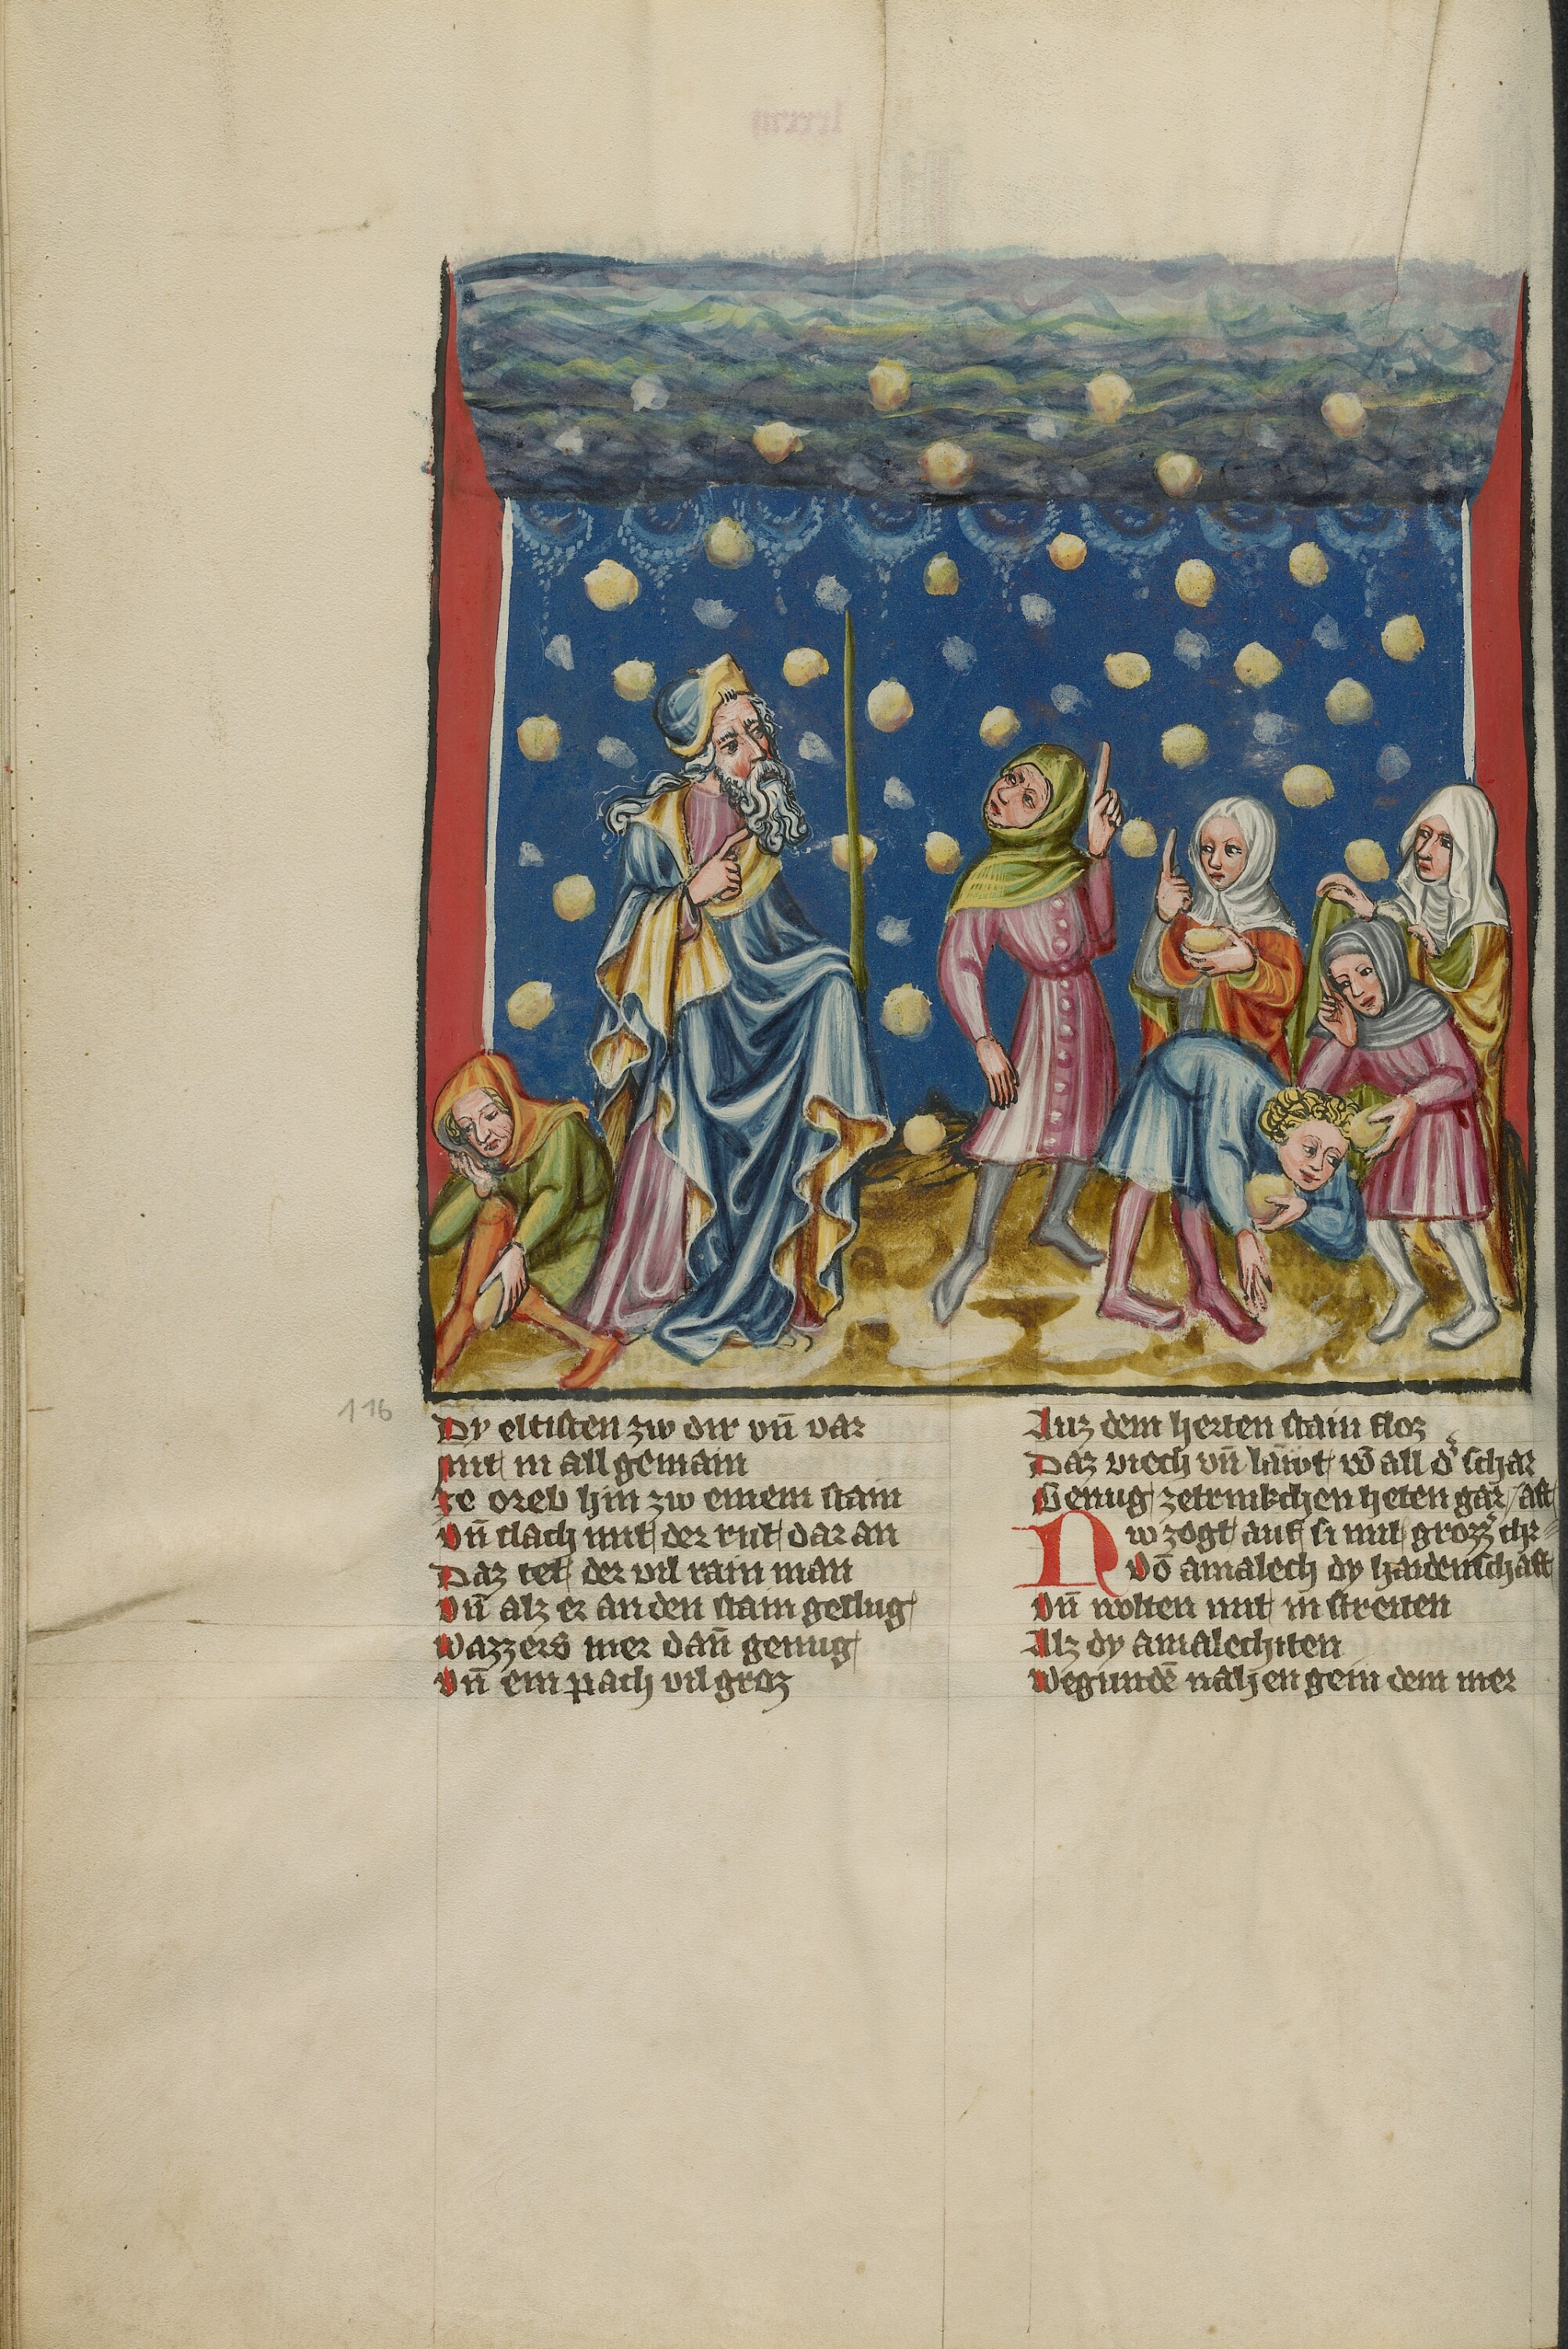
\includegraphics[height = \textheight]{figures/manna}};
\node[anchor = north east, align = right, font = \small] (title) at (1,.7) {The Israelites\\Collecting Manna\\from Heaven};
\node[anchor = north east, align = right, font = \small] (title2) at (title.south east) {Austria\\About 1400--1410};
\node[anchor = north east, align = right, font = \tiny] (title3) at (title2.south east) {Unknown artist\\Getty Open Content Program\\\href{https://www.getty.edu/art/collection/object/105T6R}{getty.edu/art/collection/object/105T6R}};
\end{tikzpicture}
\end{frame}

\begin{frame}
\huge Population Sampling
\end{frame}

\begin{frame}
\begin{tikzpicture}[x = \textwidth, y = .8\textheight]
\node (full) at (.25,.5) {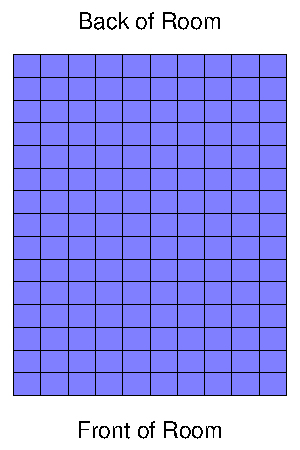
\includegraphics{figures/fullcount}};
\node<1> (srs) at (.75,.5) {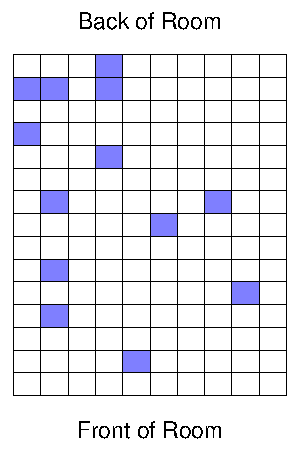
\includegraphics{figures/srs1}};
\node<2> (srs) at (.75,.5) {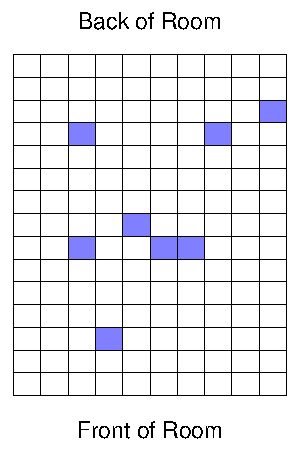
\includegraphics{figures/srs2}};
\node<3> (srs) at (.75,.5) {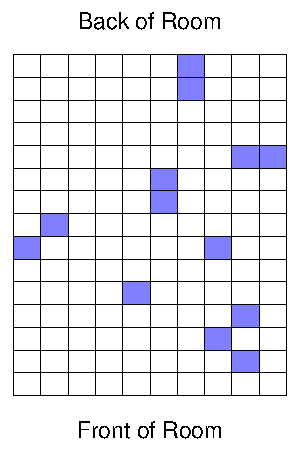
\includegraphics{figures/srs3}};
\node[anchor = south, align = center, font = \bf] at (full.north) {Full Count\\Enumeration};
\node[anchor = south, align = center, font = \bf] at (srs.north) {Probability\\Sample};
\end{tikzpicture}
\end{frame}

\begin{frame}%{Unequal probability sampling}
\begin{tikzpicture}[x = \textwidth, y = .8\textheight]
\node (design) at (.25,.5) {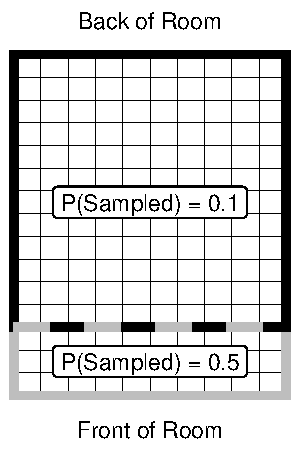
\includegraphics{figures/unequal}};
\node<1> (sample) at (.75,.5) {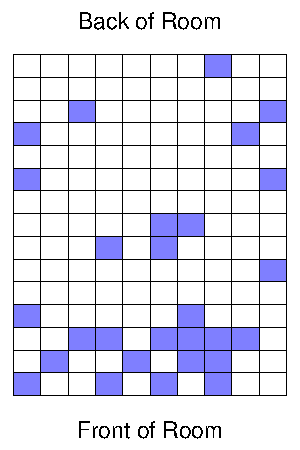
\includegraphics{figures/unequal1}};
\node<2> (sample) at (.75,.5) {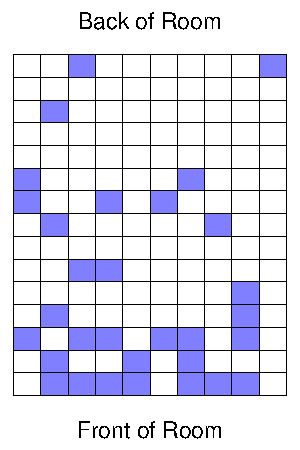
\includegraphics{figures/unequal2}};
\node<3> (sample) at (.75,.5) {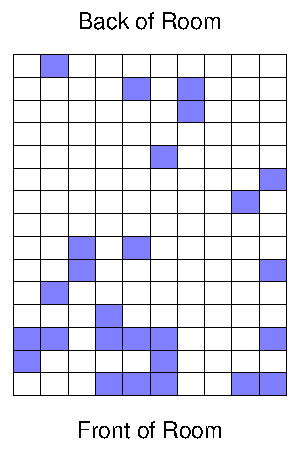
\includegraphics{figures/unequal3}};
\node[anchor = south, align = center, font = \bf] at (design.north) {Sample Design};
\node[anchor = south, align = center, font = \bf] at (sample.north) {Sample};
\end{tikzpicture}
\end{frame}

\begin{frame}
\huge Working with Data
\end{frame}

\begin{frame}{Working with Data: Finding Data}

\includegraphics[width = \textwidth]{figures/ipums_register_1.png}
\end{frame}

\begin{frame}{Working with Data: Transforming Data}
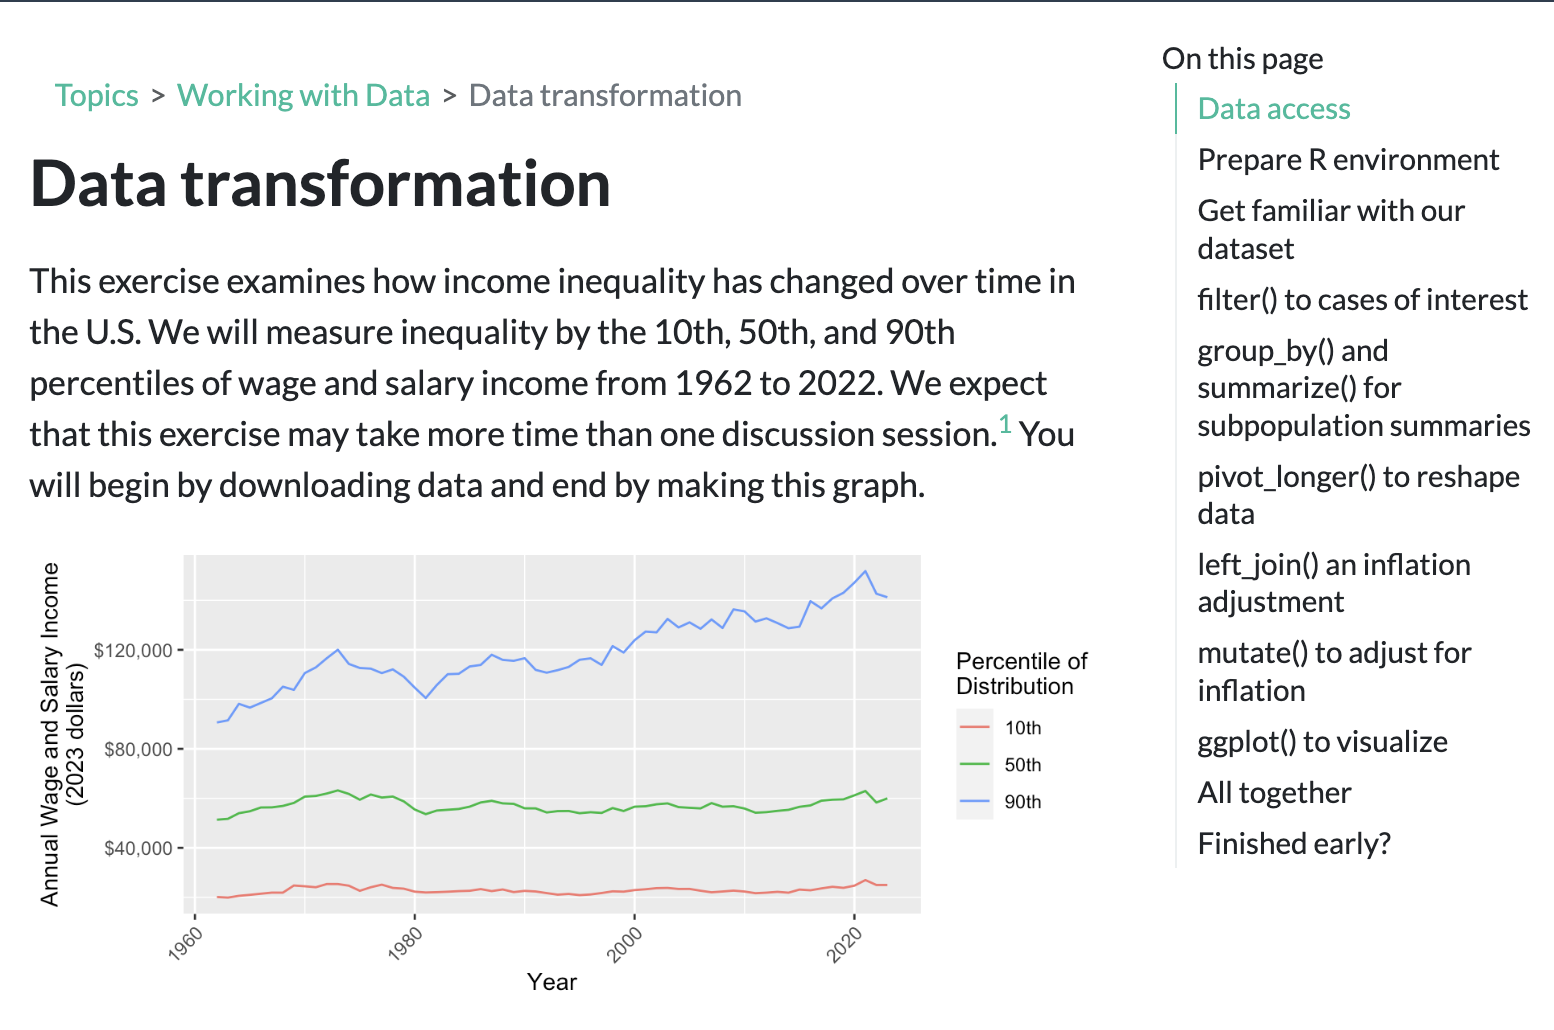
\includegraphics[width = \textwidth]{figures/transform}
\end{frame}

\begin{frame}{Working with Data: Transforming Data}

\Large 
Questions of the form: \vskip .1in
Among \_\_\_\_\_, what is the mean of \_\_\_\_\_? \vskip .3in (population inference from a sample)

\end{frame}

\begin{frame}{Working with Data: Statistical Learning}

With only the sample, estimate the mean salary of the Dodgers \vskip .2in

\begin{tabular}{ll}
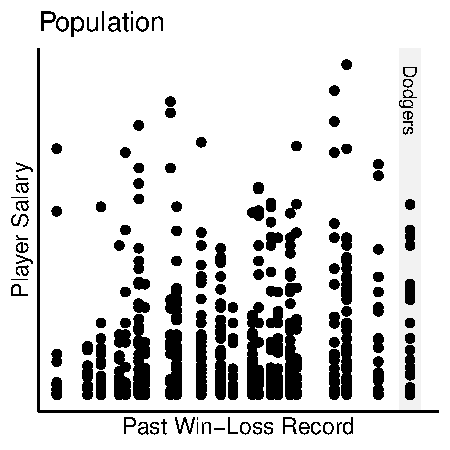
\includegraphics[width = .48\textwidth]{figures/dodgers_population} &
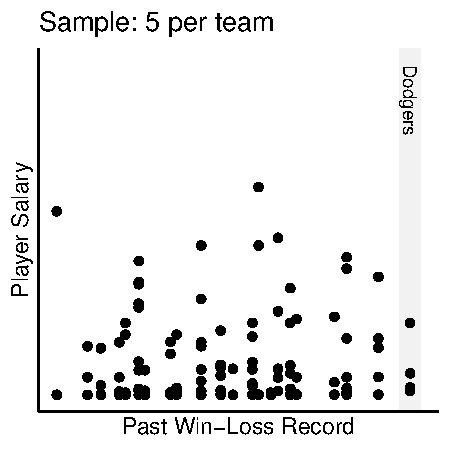
\includegraphics[width = .48\textwidth]{figures/dodgers_sample}
\end{tabular}

\end{frame}

\begin{frame}{Working with Data: Statistical Learning}

\includegraphics<1>[width = \textwidth]{figures/dodgers_estimator1}
\includegraphics<2>[width = \textwidth]{figures/dodgers_estimator2}
\includegraphics<3>[width = \textwidth]{figures/dodgers_estimator3}
\only<4->{
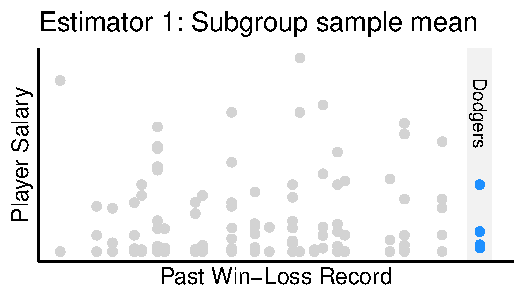
\includegraphics[width = .32\textwidth]{figures/dodgers_estimator1}
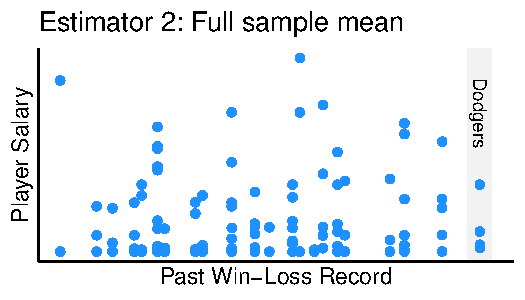
\includegraphics[width = .32\textwidth]{figures/dodgers_estimator2}
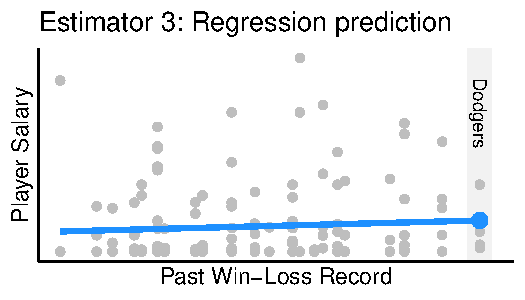
\includegraphics[width = .32\textwidth]{figures/dodgers_estimator3} \vskip .2in
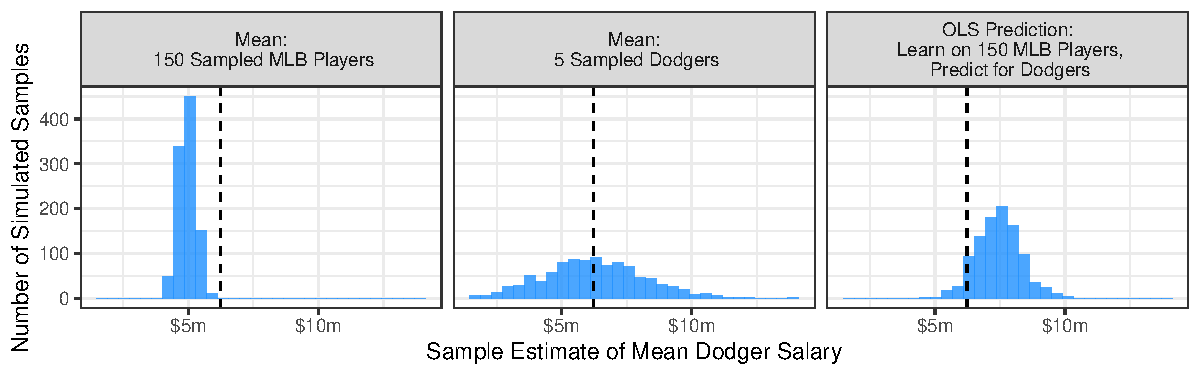
\includegraphics[width = \textwidth]{figures/dodgers_estimator_histogram}
}
\end{frame}

\begin{frame}{Working with Data: Statistical Learning}

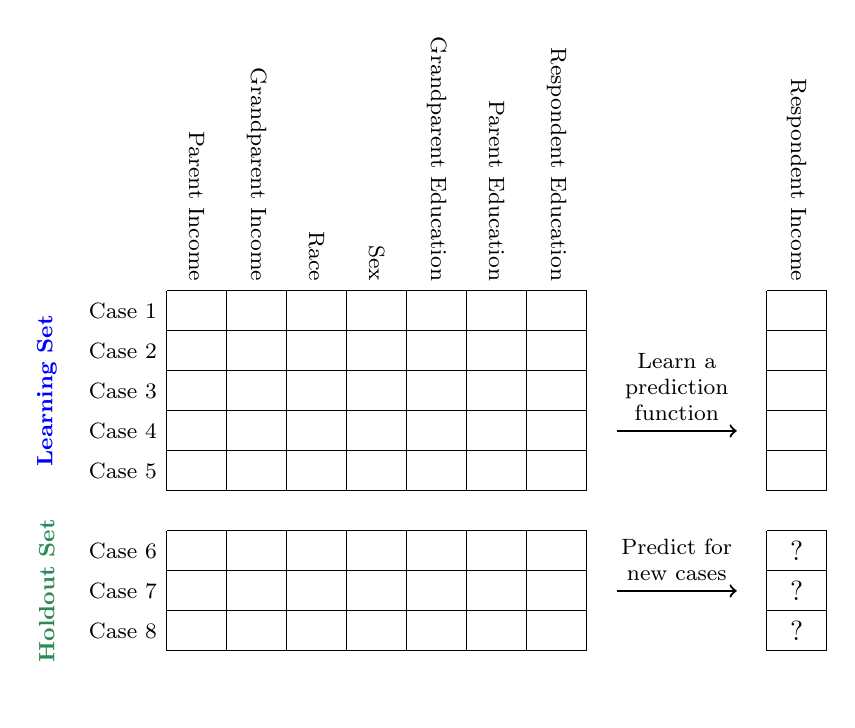
\begin{tikzpicture}[x = 3in, y = 2in]
\node[anchor = east, rotate = 270, font = \footnotesize] at (.15,1) {Parent Income};
\node[anchor = east, rotate = 270, font = \footnotesize] at (.25,1) {Grandparent Income};
\node[anchor = east, rotate = 270, font = \footnotesize] at (.35,1) {Race};
\node[anchor = east, rotate = 270, font = \footnotesize] at (.45,1) {Sex};
\node[anchor = east, rotate = 270, font = \footnotesize] at (.55,1) {Grandparent Education};
\node[anchor = east, rotate = 270, font = \footnotesize] at (.65,1) {Parent Education};
\node[anchor = east, rotate = 270, font = \footnotesize] at (.75,1) {Respondent Education};
\node[anchor = east, font = \footnotesize] at (.1,.95) {Case 1};
\node[anchor = east, font = \footnotesize] at (.1,.85) {Case 2};
\node[anchor = east, font = \footnotesize] at (.1,.75) {Case 3};
\node[anchor = east, font = \footnotesize] at (.1,.65) {Case 4};
\node[anchor = east, font = \footnotesize] at (.1,.55) {Case 5};
\draw[step=.1,black,thin] (0.1,.5) grid (.8,1); 
\node at (.5,1) {};
\node[anchor = east, rotate = 270, font = \footnotesize] at (1.15,1) {Respondent Income};
\draw[step=.1,black,thin] (1.1,.5) grid (1.2,1);
\draw[thin] (1.2,.5) -- (1.2,1);
\draw[->, thick] (.85,.65) -- node[midway, above, font = \footnotesize, align = center] {Learn a\\prediction\\function} (1.05,.65);
% Holdout set
\draw[step=.1,black,thin] (0.1,.1) grid (.8,.4);
\draw[step=.1,black,thin] (1.1,.1) grid (1.2,.4);
\draw[thin] (1.2,.1) -- (1.2,.4);
\node at (1.15,.35) {?};
\node at (1.15,.25) {?};
\node at (1.15,.15) {?};
\node[anchor = east, font = \footnotesize] at (.1,.35) {Case 6};
\node[anchor = east, font = \footnotesize] at (.1,.25) {Case 7};
\node[anchor = east, font = \footnotesize] at (.1,.15) {Case 8};
\draw[->, thick] (.85,.25) -- node[midway, above, font = \footnotesize, align = center] {Predict for\\new cases} (1.05,.25);
% Label the two
\node[rotate = 90, font = {\footnotesize\bf}, blue] at (-.1,.75) {{Learning} Set};
\node[rotate = 90, font = {\footnotesize\bf}, seagreen] at (-.1,.25) {{Holdout} Set};
\node at (-.05,0) {};
\end{tikzpicture}
\end{frame}

\begin{frame}
\huge Describing Inequality
\end{frame}

\begin{frame}{Describing inequality: We practiced descriptive research questions}

\begin{itemize}
\item race: the median white household has \$5.48 for each \$1 held by the median Black household
\begin{itemize}
\item and we discussed political origins
\end{itemize} \pause
\item gender: ``the ratio of women's pay to men's pay increased from 0.61 to 0.83 between 1970 and 2018''
\begin{itemize}
\item from England et al. 2020, in Problem Set 2
\end{itemize} \pause
\item class: professional workers have higher incomes if their parents were also professional workers
\begin{itemize}
\item Laurison \& Friedman 2024, in Problem Set 4
\end{itemize}
\end{itemize}

\end{frame}

\begin{frame}
\huge Reducing Inequality
\end{frame}

\begin{frame}{Reducing Inequality: Moral Arguments}
What would make a distribution just? \pause
\begin{itemize}
\item We'd choose it in the original position \hfill (Rawls) \pause
\item It arises through just acquisitions and just transfers \hfill (Nozick)
\end{itemize}
\end{frame}

\begin{frame}
\includegraphics[width = \textwidth]{figures/holc-scan-la}
Source: Nelson and Ayers, \bref{https://dsl.richmond.edu/panorama/redlining/}{Mapping Inequality}
\end{frame}

\begin{frame}
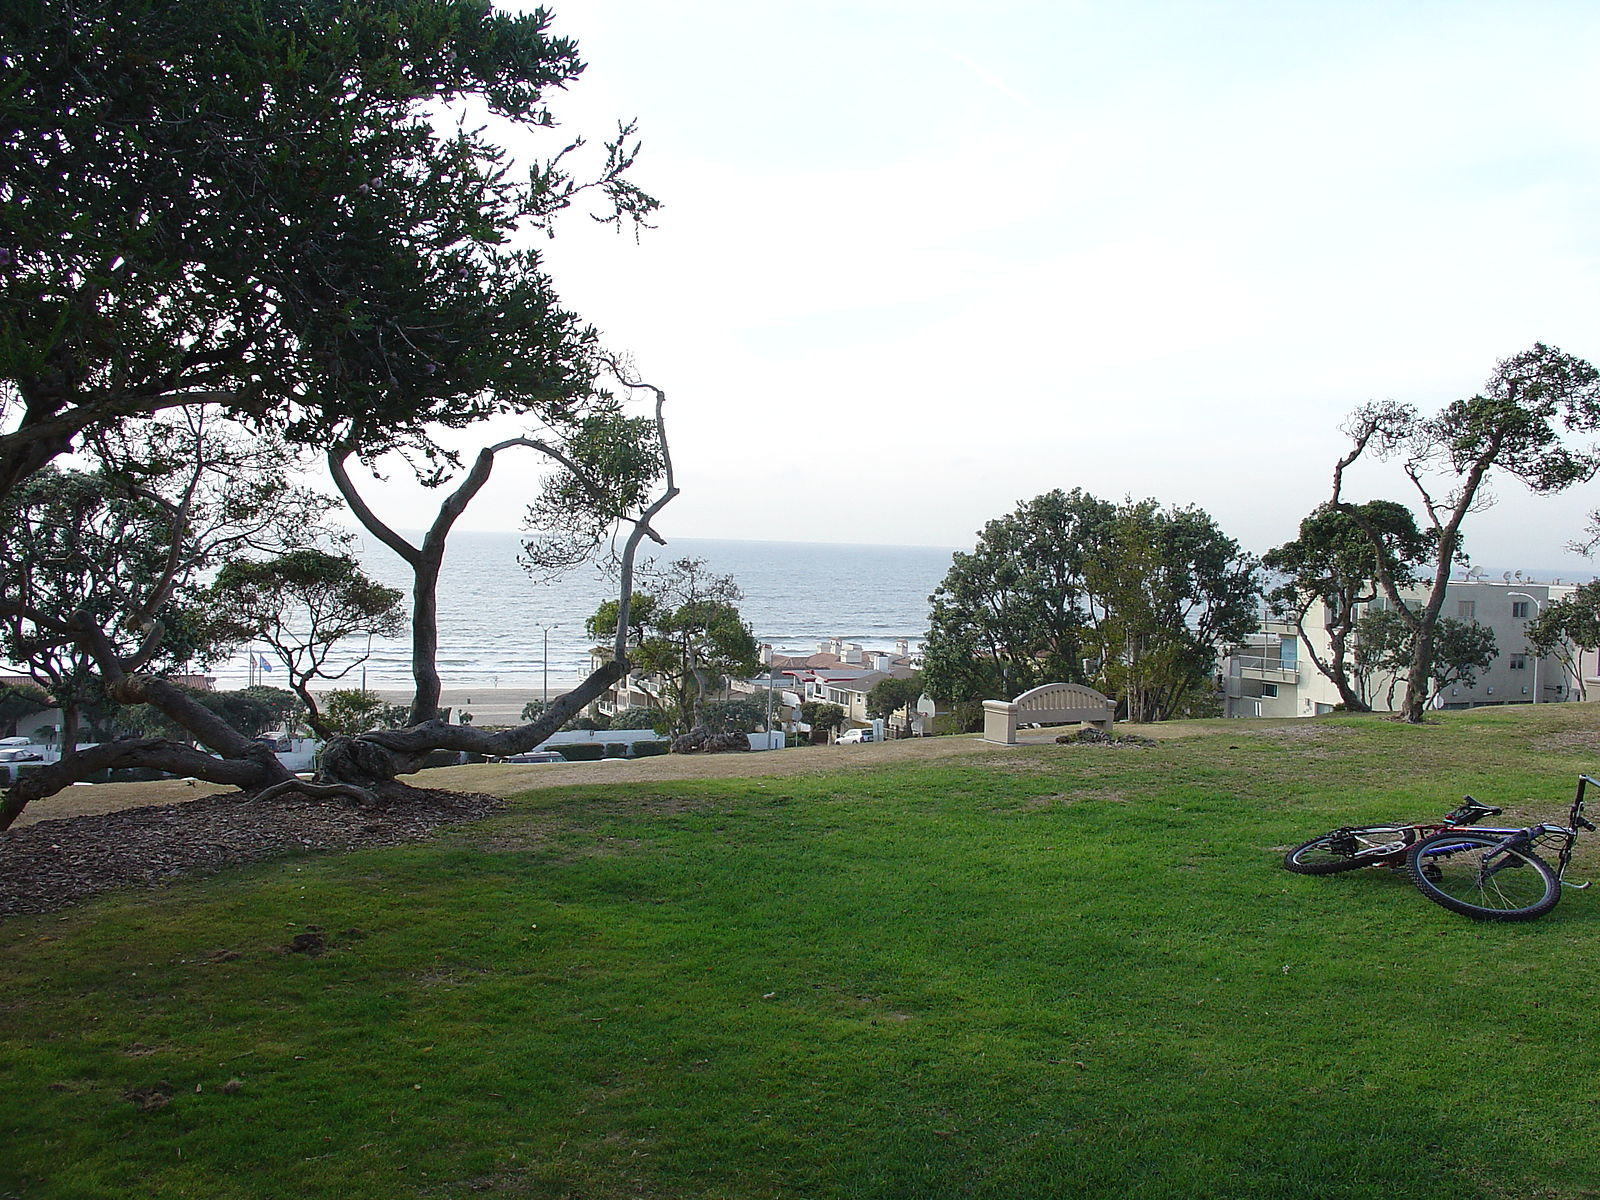
\includegraphics[width = \textwidth]{figures/park}\\
Source: Wikimedia
\end{frame}

\begin{frame}
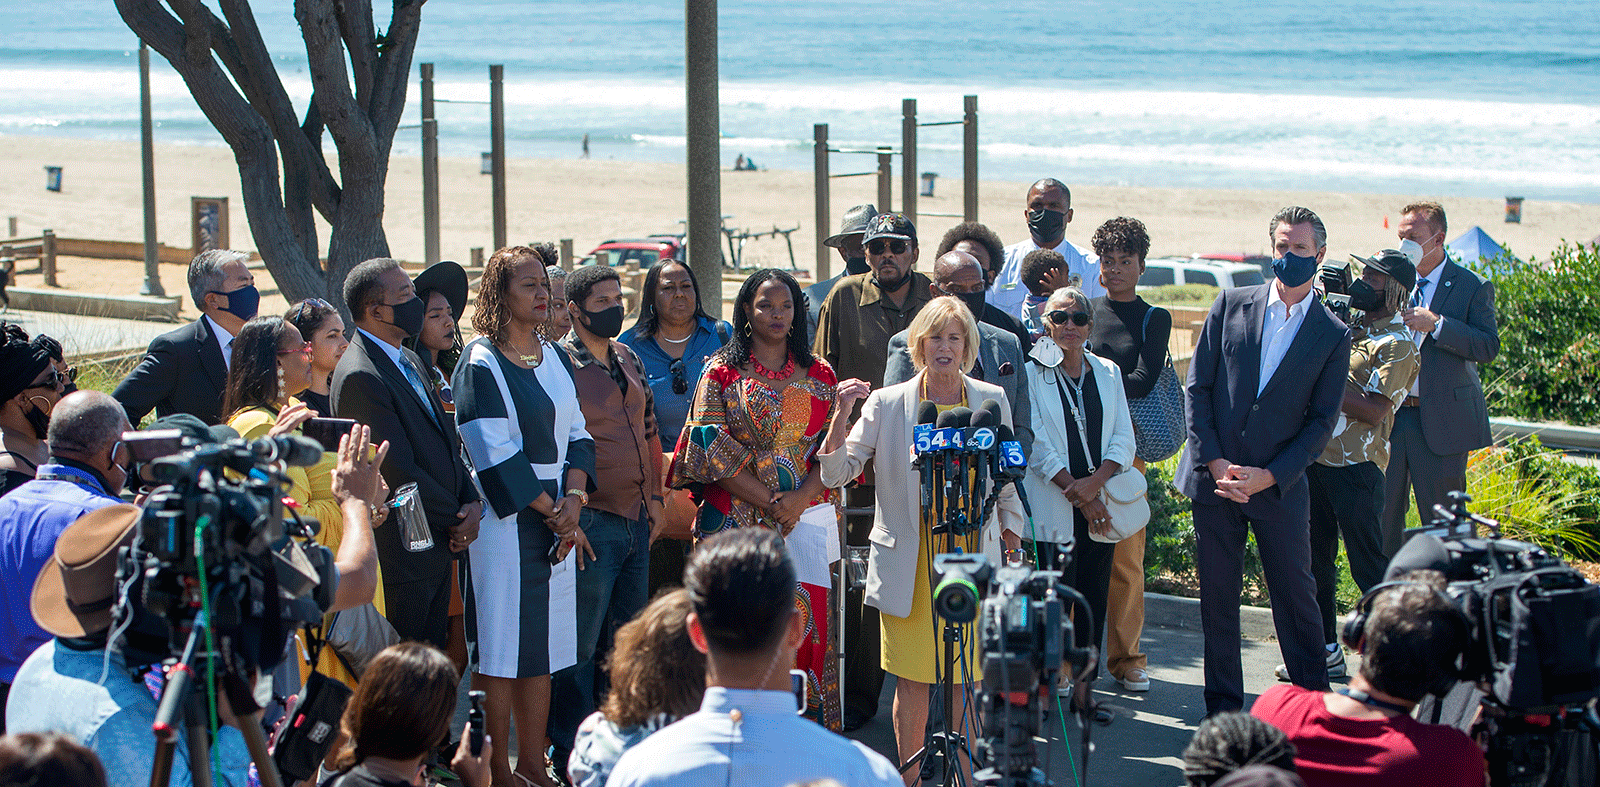
\includegraphics[width = \textwidth]{figures/reparation} \\
Source: \href{https://ceo.lacounty.gov/ardi/bruces-beach/}{County of Los Angeles}
\end{frame}

\begin{frame}
\huge Reducing Inequality:\\Causal Inference
\end{frame}

\begin{frame}{Two claims}


\begin{tikzpicture}[x = \textwidth, y = .8\textheight]
\node at (0,0) {};
\node at (1,1) {};
\node[anchor = north west, align = left] at (.05,1) {People with\\college degrees\\earn more};
\node[anchor = north west, align = left] at (.55,1) {A college degree\\causes\\higher earnings};
\draw[rounded corners, fill = blue, fill opacity = .3] (.05,.3) rectangle (.25,.5) {};
\draw[rounded corners, fill = seagreen, fill opacity = .3] (.25,.1) rectangle (.45,.3) {};
\node[anchor = north, align = center, font = \footnotesize, blue] at (.15, .1) {Outcome\\with college};
\node[anchor = north, align = center, font = \footnotesize, seagreen] at (.35, .1) {Outcome\\without};
\node[anchor = south, rotate = 90, align = center] at (.05, .3) {People};
\draw[rounded corners, fill = blue, fill opacity = .3] (.55,.1) rectangle (.75,.5) {};
\draw[rounded corners, fill = seagreen, fill opacity = .3] (.75,.1) rectangle (.95,.5) {};
\node[anchor = north, align = center, font = \footnotesize, blue] at (.65, .1) {Outcome\\with college};
\node[anchor = north, align = center, font = \footnotesize, seagreen] at (.85, .1) {Outcome\\without};
\node[anchor = south, rotate = 90, align = center] at (.55, .3) {People};
\node at (.15, .4) {$Y_i$};
\node at (.35, .2) {$Y_i$};
\node at (.65, .3) {$Y_i^\text{College}$};
\node[font = \small] at (.85, .3) {$Y_i^\text{Non-college}$};
\node[anchor = north, align = center] (factual) at (.25,.7) {factual\\outcomes};
\draw[->, thick] (.2,.55) -- (.15,.45);
\draw[->, thick] (.3,.55) -- (.35,.25);
\node[anchor = north, align = center] (potential) at (.75,.7) {potential\\outcomes};
\draw[->, thick] (.7,.55) -- (.65,.35);
\draw[->, thick] (.8,.55) -- (.85,.35);
\node[anchor = north east, align = right, font = \footnotesize, gray] at (1,.7) {\href{https://catalog.library.cornell.edu/catalog/12108069}{Imbens \&}\\\href{https://catalog.library.cornell.edu/catalog/12108069}{Rubin}\\\href{https://catalog.library.cornell.edu/catalog/12108069}{2015}};
\end{tikzpicture}

\end{frame}

%\begin{frame}
%\includegraphics[width = \textwidth]{figures/dag_slide}
%\end{frame}

\begin{frame}
\huge Final Project
\end{frame}

\begin{frame}{What we did in this course}
\begin{enumerate}
\item Population Sampling
\item Working with Data
\item Describing Inequality
\item Reducing Inequality
\end{enumerate}
leading to your own final projects
\end{frame}

\begin{frame}{\bblue{Feedback} }

\large 
\begin{enumerate}
\item What will you walk away now able to do?
\item What worked especially well?
\item How could this course be even better?
\end{enumerate}
\end{frame}

\begin{frame}{Course evaluations} \pause

\begin{itemize}
\item Specific examples are especially helpful
\begin{itemize}
\item Comments on course content
\item Comments on course delivery
\end{itemize} \pause
\item Specific positive experience with a TA? Tell us by name!
\end{itemize}

\end{frame}

\begin{frame}
\huge Thank you for a great semester!
\end{frame}

\end{document}